\begin{graphicspathcontext}{{./chapters/sarl/imgs/},{./chapters/sarl/imgs/auto/},\old}

\begin{frame}{What is a Holon?}
	\begin{columns}[T]
		\begin{column}{.6\linewidth}
			\begin{block}{Origin \cite{koestler67}}
				A \emph{holon} is something that is \emph{simultaneously}:
					\begin{description}
					\item [whole] it has its own identity and autonomy
					\item [part]  it belongs to a larger whole
					\end{description}
			\end{block}
			\vspace{.5cm}
			\begin{example}
				Think of a \emph{cell} in a body:
				\begin{itemize}
				\item it lives, acts, and decides on its own
				\item yet it is a component of a tissue, an organ, an organism
				\end{itemize}
			\end{example}
			\vspace{.5cm}
		\end{column}
		\begin{column}{.4\linewidth}
			\begin{alertblock}{Key idea for SARL}
				Every SARL agent is a holon. \\
				The terms \emph{agent} and \emph{holon} are synonymous in SARL
			\end{alertblock}
			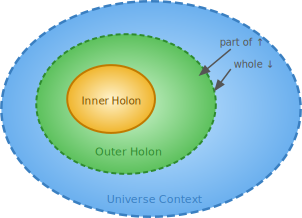
\includegraphics{sarl_holon_concept}
		\end{column}
	\end{columns}
\end{frame}

\begin{frame}[t]{Context: Shared Space between Agents}
	\begin{columns}
		\begin{column}{.5\linewidth}
			\smaller
			\begin{definitionblock}{Context}
				A \emph{context} is a shared environment in which agents live
			and interact.
				\begin{itemize}
				\item It contains one or more \emph{spaces} (interaction channels)
				\item Every context has a mandatory \emph{default space}
				\item Agents in the same context can exchange events through that default space
				\end{itemize}
			\end{definitionblock}
			\vspace{.25cm}
			\begin{block}{Two kinds of contexts for an agent}
				\begin{description}
				\item[Default context] the context in which the agent was spawned. It is its "social" environment
				\item[Inner context] the context \emph{owned} by the agent itself. Sub-agents live here
				\end{description}
			\end{block}
		\end{column}
		\begin{column}{0.5\linewidth}
			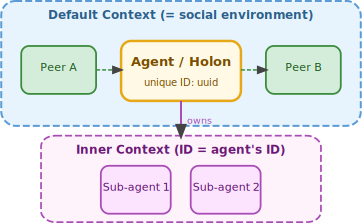
\includegraphics{sarl_agent_contexts}
		\end{column}
	\end{columns}
\end{frame}

\begin{frame}{{Inner Context:} agents inside agents}
	\smaller
	\begin{columns}
		\begin{column}{0.52\textwidth}
			\begin{block}{Every agent owns an inner context}
				\begin{itemize}
				\item An agent can \emph{spawn sub-agents} inside its own inner context
				\item The sub-agents are called \emph{sub-holons}
				\item The spawning agent becomes the \emph{super-holon} (or super-agent)
				\item The unique ID of the inner context equals the ID of its owning agent
				\end{itemize}
			\end{block}
			\hiconbox{
				An agent is \emph{always} a member of the default space of its \textbf{own inner context} \newline
				$\Rightarrow$ it can communicate with its sub-agents through that space
			}{info-icon}
		\end{column}
		\begin{column}{.5\linewidth}
			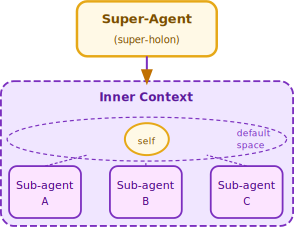
\includegraphics{sarl_inner_context}
		\end{column}
	\end{columns}
\end{frame}

\begin{frame}[t]{Holarchy: a Hierarchy of Holons}
	\smaller
	\begin{columns}
		\begin{column}{0.55\textwidth}
			\begin{definitionblock}{Holarchy \cite{koestler67}}
				A \emph{holarchy} is a recursive hierarchy of holons
				\begin{itemize}
				\item Each level is both a \emph{whole} (for the level below)
				and a \emph{part} (for the level above)
				\item The structure can be as deep as needed
				\end{itemize}
			\end{definitionblock}
			\begin{block}{At the top: the Universe Agent}
				\begin{itemize}
				\item \emph{Universe Agent} is the root of every holarchy
				\item Its inner context is the \emph{Universe Context} (called \emph{Janus Context} in the Janus runtime)
				\item All first-level agents are spawned inside it
				\end{itemize}
			\end{block}
			\begin{example}{Self-similarity}
				Each agent has the \emph{same structure}: it can always act as a simple agent \emph{and} as a container of other agents
			\end{example}
		\end{column}
		\begin{column}{.5\linewidth}
			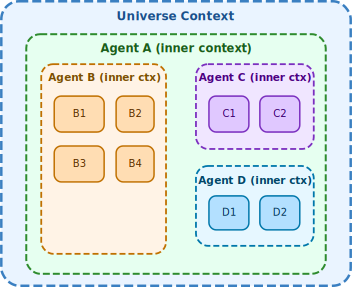
\includegraphics{sarl_holarchy}
		\end{column}
	\end{columns}
\end{frame}

\begin{frame}[fragile]{{SARL in Practice:} Super-Agent and Sub-Agent}
	\smaller
	\begin{columns}
		\begin{column}[t]{.5\linewidth}
			\Emph{Defining a sub-agent:}
			\begin{sarllisting}[basicstyle=\tiny]
agent Worker {
	uses Logging
	on PerformTask {
		// react to a task
		info("Task done!")
	}
}
			\end{sarllisting}
			\Emph{Defining the super-agent:}
			\begin{sarllisting}[basicstyle=\tiny]
agent Manager {
	uses Lifecycle
	uses InnerContextAccess

	on Initialize {
		// spawn a sub-agent
		// inside inner context
		spawnInContext(
			Worker,
			innerContext)
	}
}
			\end{sarllisting}
		\end{column}
		\begin{column}[t]{.5\linewidth}
			\Emph{Sending an event downward:}
			\begin{sarllisting}[basicstyle=\tiny]
agent Manager {
	uses Behaviors

	def requestTask {
		// wake sub-agents
		// via inner context
		wake(new PerformTask)
	}
}
			\end{sarllisting}
			\Emph{Sending an event upward:}
			\begin{sarllisting}[basicstyle=\tiny]
agent Worker {
	uses DefaultContextInteractions

	on TaskDone {
		// forward to parent
		occurrence.emitToParent
	}
}
			\end{sarllisting}
		\end{column}
	\end{columns}
\end{frame}

\end{graphicspathcontext}

\endinput

